\documentclass{article}
\usepackage{graphicx}
\usepackage[margin=1in]{geometry}
\parskip=2mm
\title{Coursework 1: Methods and Plans}
\author{Group 31}
\begin{document}
\maketitle
The project which we were assigned was initially entitled “Eye Capture Window Manager”.  The aim of which is to create a piece of window management software that integrates with a linux operating system.  This should use eye tracking to monitor the user’s gaze and in turn which window is being observed and switch focus accordingly.
\section*{Agile Method}
We examined the agile methods that were presented to us, and having weighed the pros and cons of each decided to choose Kanban.  This is because Kanban is more flexible than the methodologies of XP or Scrum, as they are both more prescriptive in personnel roles, frequency and purpose of meetings and rigid practices that must be kept to every iteration.  In contrast, the Kanban board seems like a very flexible and  incredibly useful tool in tracking the development cycle of features and learning how this can be made more efficient: finding the bottlenecks in the process.  Having this visualisation means that all members of the team know where each feature is in the development process.  No member of the team has a particularly large specialisation in a certain area, so this means everybody can be involved, to a certain extent, on the implementation of each feature when need be. It is also markedly different to the methodologies that most members of the group have used in previous group projects, and therefore provides a good opportunity to try something new to increase productivity.

The potential scope of the project is very large, but our team has a strictly limited set of resources to complete it.  This is another reason we chose Kanban, as its limit of the amount of work in progress at a particular time means the team will not be overwhelmed with features in the development process.   Without a similar methodology, our fear was we could end up with many partly implemented features and an unfinished product. With it, we should be able to focus on the things we need to get working first, then move onto the smaller and perimeter features,

Another important aspect of our project is that nobody in our team, or even our Supervisor, have a particular idea of how difficult or time consuming each step will be. Kanban encourages constant small changes over time in comparison to larger changes in one sprint or cycle.  This means the project, which is still young and we are yet to fully understand, will be agile to changing requirements which we will most definitely encounter as we begin to implement.

\clearpage
We are using the website ‘Trello’ as a Kanban board to track the progression of features through the development cycle.  While this website is not specifically designed for this purpose, it provides the facilities to do so: columns in which tasks can be pinned and dragged from one to the other.  The categories we are currently using are named as follows:

\begin{itemize}
\item TODO: features that are yet to be started
\item Analysis: analysing how the feature should be implemented
\item Doing: features currently in development
\item QA: features going through testing
\item Done: features that are complete, left on the board in case future issues occur that move them back down
\end{itemize}

The screenshot included shows our current project on the website with a couple of cards added. \\[1mm]

{\centering
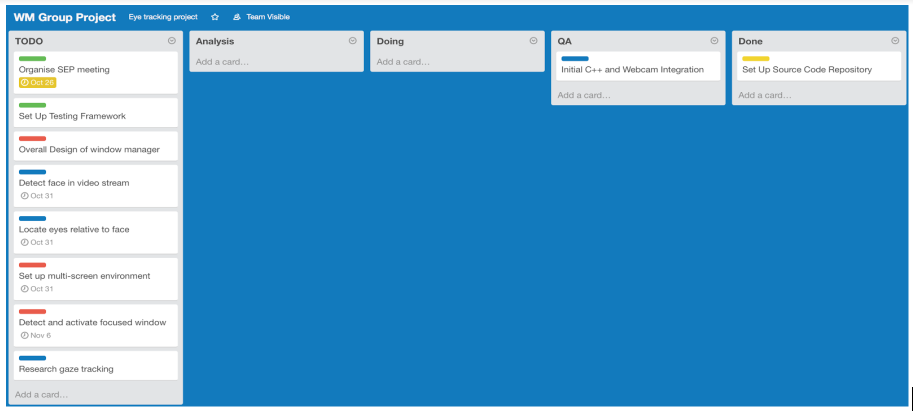
\includegraphics[scale=0.45]{trello.png}\par
}

\vspace{1mm}
We chose to use this site as our Kanban board as, whilst it lacks some useful features (maintaining links between cards for dependencies for example) it is much smoother and more reliable as a user experience than many competitors. We carefully looked at Volerro as a direct comparison, but came across many small bugs during our experiments which made the experience much less enjoyable. 

The team still has regular meetings in addition to subscribing to the Kanban methodology.  This allows face-to-face time with the group which is useful for having more complex discussions related to development or other issues.  A diary is kept of tasks achieved and problems encountered during these meetings so we have a history of how the project has progressed and how we have managed to deal with issues that we have encountered.

\clearpage
\section*{Engineering Plan}
We have split the group into 2 even sized sub teams (3 members each), one working on the eye tracking and the other working on switching windows/window management and user interface. This split makes sense in our context for two main reasons. First, the project is easily divisible (the two sides ought to be isolated anyway to maximise the potential of them both) and both sides will require large amounts of work from the start. In addition, 3 members of the group are taking the Computer Vision course which will both support and be supported by the project, while the other members have chosen other options this term, which could potentially lead to problems in the more intensive areas of the eye tracking side of the project. Having said this, we anticipate the eye tracking to take longer, so the assignment of the subteams is flexible. 

This division lead us to the conclusion we should create two fairly separate programs, sharing very little, if any, internal details. The window team will have to provide an interface to change the focus of windows, and will design the communication between the apps. The eye tracking app will detect the user gaze, and convert its conclusions into messages to the window app. Splitting the implementation in this way allows the potential to use the components separately, for instance using the eye tracking system with other operating systems or other display servers, or building a system that detects another physical input which can change the focus of windows and be managed in the same way.

\subsection*{Eye Tracking}
The plan is to start by tracking the user's face in order to detect which screen they are looking at. From meetings with our supervisor, we were directed to Aldo Faisal who has done previous work in areas similar to this. Due to his experience, he advised us that we should start with simple face detection rather than the precision of detecting the user’s gaze.  The “Viola-Jones” technique is one that was specifically motivated by the problem of face detection.

We expect to be able to use just a webcam for the face tracking and hope to continue without any extra equipment to track the user’s eyes. However our research has shown that using an infrared light source to illuminate the user’s eyes would allow the easier detection of the eyes due to the bright pupil effect. So we will evaluate the cost and availability compared to the benefit provided, aiming to use low cost, off the shelf equipment. As we move into the development and encounter these problems, we will be much better placed to work out whether we need to employ less standard hardware.

Development on this side has started by researching a library to use for the video processing. We discovered and decided to use the C++ library OpenCV, as it handles integration with multiple webcams, an interface to substitute video or photos in place of a webcam, defines easy to use templates for handling images, and even implements some of the image processing techniques we may need to use. We have successfully managed integration with a webcam, live frame by frame processing of the video stream it provides, and use of the GUI library that pairs with OpenCV (called highgui) to display the feed. We now plan to start working on face detection, and then inferring which direction a user is looking. Hopefully, this should be complete by week 6, but as none of us have done anything similar in the past, estimating these things is quite hard.

Once face detection by “Viola-Jones” is complete, we plan to look into more precise detection of where the user is looking. This will take three things: The detection of the eye, the tracking of the eye, and inferring where the eye is pointing. The first part, eye detection, can be tried on still images and should use many of the features that openCV provides. It may need some experimentation and iteration to complete, as there are many methods people successfully employ depending on conditions and requirements. The second part of eye tracking management takes the form of tracking a detected eye frame to frame. As the position of the eye is known initially, it should be easier to locate in the next frame, allowing us to save a lot of computation.  The final part relies on the completion of the first two, and suggests the use of a lot more techniques to get the detection of exact gaze position from the images. We plan to have at least some increase in precision of gaze position inference (over just using face/head position) by the end of term, and will hopefully try to continue improving it over the christmas holidays. Cursory research has shown existing methods that track the pupil relative to another point such as a corneal reflection, but we need to do a lot more research on the best potential techniques.

\subsection*{Window Management}
The team working on window management will work in parallel with the eye tracking team, but we anticipate that it will be a faster set of tasks to complete. The aim will be to convert eye tracking data from a camera into switching the focused window. Initially, we will only know which side of the camera the user’s gaze is, and with the camera will be placed between two monitors, we will be able to activate the last used window on the monitor being looked at. As the eye tracking team gain more precision, the precision of selecting windows will need to increase.

Our initial thought was to build our own window manager on top of one with basic functionality, such as TinyWM.  This allows us to add the features that we want without having to build the window manager from scratch.  Therefore, we can align the windows exactly as we wish making the testing of features more simple.  However, after further researching the implementation of linux window management (XServer and Xlib) we found that it may be simple to allow this functionality on a wide variety of window managers.  This would mean users could use their own window manager rather than one we developed ourselves. We will be focusing on tiling window managers in the development, as the rigidly defined regions are more appropriate for our software, but we won’t rule out testing on floating window managers if time allows.

The timescale for the task is still fairly fluid as we are unsure exactly how long each feature will take. However, the libraries that are used for changing focus in the screen are well documented and unlike movement tracking, not experimental. Thus iteration should be fairly rapid and new functionality should grow steadily through the project timeline.

The task will need to take the information which has been gathered on the direction of the user’s gaze and change the window/screen which is in focus accordingly. Since there will not be any eye tracking data for much of the project, the Window Manager will be unit-tested using mock data. It will connect to the eye tracking part once eye tracking is implemented. We also think it will be useful for the sensitivity level to be modifiable, so these unit tests should be able to test that functionality as well.

\subsection*{User Interface}
Once the Eye Tracking and Window Management have been completed - we will create a User Interface to enable, disable and manage configurations of the software, such as monitor positioning and potentially some user-input for calibrating the eye tracking software. Since it is the last thing we will do, it is likely the UI will be done by the Window-Manager subteam, since we expect that part of the project to take less time. It will most likely be done during the Christmas holidays, during the last few weeks of the project. As it will also just be hooking into functions that we will need to exist anyway, and will simply replace, for example, a configuration file, it should be fairly simple to implement.

\clearpage
At this early stage, it’s hard for us to work out what we are going to want to configure fully, but we have made a mock-up of what the configuration of some of the parameters could look like: \\[1mm]

{\centering
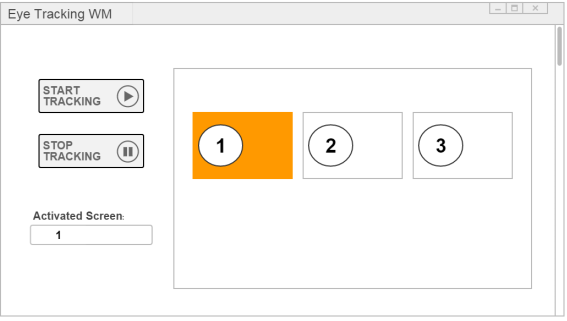
\includegraphics[scale=0.7]{ui.png}\par
}

\end{document}
